\section{Death and Final Judgment}

\begin{wrapfigure}{rt}{.3\textwidth}
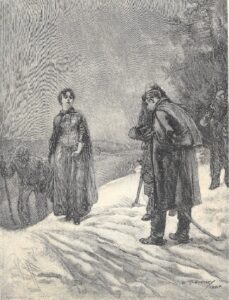
\includegraphics[width=.25\textwidth]{I_come_to_claim_my_dead-229x300.jpg}
\end{wrapfigure}

\begin{quotex}
Arseny's soul wanted to touch Ursina's soul ... Get used to separation, said Death, it is painful, even if it is only temporary. Will we recognize each other in eternity? asked Arseny's soul. That depends in large part on you, said Death: souls often harden during the course of life and then they barely recognize anyone after death.
\flright{\textsc{Eugene Vodolazkin}, \emph{from Laurus}}
\end{quotex}


\paragraph{Potter's Field}

\begin{quotex}
The potter's field was a mournful place... There lay the plague dead, pilgrims, the strangled, unbaptized babies, and suicides; those drowned by waters, taken by battle, murdered, and stricken by fire. Suddenly surprised, those who had fallen from lightning, dead from frost and every sort of wound. The lives of those unfortunates were varied and it was not life that united them: their resemblance to one another consisted of death. It was death without Confession.
\flright{\textsc{Eugene Vodolazkin}, \emph{from Laurus}}
\end{quotex}


That was the situation in Russia, some six centuries ago. Potter's field was an open pit into which the corpses were dropped. Once a year, a priest gave a blessing, the pit was filled in, and another one dug.

If sudden death without benefit of the last sacraments is a curse, then presumably a slow death, preceded by a gradual breakdown of organs, must be a blessing.

A few years ago I was sitting across the desk of a specialist. He looked at my medical history and test results, then looked up at me. He read another page and looked up again. Finally, after he had read the full report, he said to me, ``Well, at least you \emph{look} good!''

\paragraph{Genetics and the Gods}


Evolutionary psychology asserts, without proof, that the existence of some deviant behavior must have had some survival value. But that is precisely the pagan view: whatever is, must have been willed by the gods.

Obviously that is both bad science and bad theology. Whatever genetic features (assuming even that it is genetic) exists is not necessarily selected. Rather it could be mutations that have not been eradicated. Deleterious mutations in the genetic code, or ``genetic load'', are always arising. Moreover, there may be group selections: a disordered society may select for various psychological disorders.

True Providence is the Realm of Being, of possibilities of manifestation, the world of perfection. That is what God wills. The Realm of Existence, or Becoming, is less certain. Therefore, it requires discernment to determine the will of God in any situation.

\paragraph{Detachment from the World is Attachment to God}


I listened to an online sermon with the title Detachment from the World is Attachment to God\footnote{\url{https://www.youtube.com/watch?v=4Oo8HO1obOo}}.

Thanks to youtube matching, it pulled up a lecture by a yogi with the same title. It was not in English, so I don't know what was said. I assume the point was the same.

\paragraph{The Last Judgment}


\begin{quotex}
He sitteth on the right hand of the Father, God Almighty, from whence he shall come to judge the quick and the dead. At whose coming all men shall rise again with their bodies, and \emph{shall give account for their own works}.
\flright{\textsc{from the Athanasian Creed}}

Before this throne, in my vision, the dead must come, great and little alike; and the books were opened. Another book, too, was opened, the book of life. And the dead were judged by their deeds, as the books recorded them.
\flright{\textsc{Revelation 20:12}}

The just shall appear whiter, more beautiful, and more resplendent than the sun. ... on the other hand, the bodies of the reprobate shall appear black and hideous, and shall send forth an intolerable stench.
\flright{\textsc{St. Alphonsus Liguori}, \emph{Preparation for Death}}
\end{quotex}


According to the saints, the general judgment is the third coming of Christ, not the second that is commonly supposed. At that time, all souls will be exposed: some will be pure, most will be hardened and barely recognizable.

The purpose is to demonstrate the justice of the judgment. The consequences of one's thoughts, words, and deeds will be fully revealed. In our current condition, we can seldom see them beyond a few people close to us or a few years in the future. However, in the general judgment, we will see how our thoughts, words, and deeds rippled through the world and down through the generations. One bad choice now may be felt for several generations.

Our innermost thoughts will be exposed. Perhaps you lusted after your neighbor's wife, or worse, his daughter, or even worse, your own step-daughter. Maybe you gossiped about or harshly criticized a friend or relative behind his back; that will all become known. You get the picture. The point is to prepare for it by keeping your soul pure right now.

You say you don't believe in such superstitions. Does that really make it OK? Do you really mean that you can lust, hate, steal, or bring pain just because no one will ever find out? That is really sad. You would be better off believing the superstition than believing your own denials, lies, and self-deception.

\begin{quotex}
How could there be light for the man who obstinately rejects the light and how would there be salvation for the man who is convinced that he must be saved from nothing and nobody has to be saved in the inexplicable drama of life? God cannot give himself to those who do not want Him, to insist with those who are deaf and blind. Religion requires men of good will who adhere to and want to adhere to the Law of God. Whoever rejects it is judged by himself before being judged by God.
\flright{\textsc{Guido Di Giorgio}}
\end{quotex}



\flrightit{Posted on 2020-02-28 by Cologero}


